%%%%%%%%%%%%%%%%%%%%%%%%%%%%%%%%%%%%%%%%%%%%%%%%%%%%%%%%%%%%%%%%%%%%%%%%%%%%%%%%
%
% Template license:
% CC BY-NC-SA 3.0 (http://creativecommons.org/licenses/by-nc-sa/3.0/)
%
%%%%%%%%%%%%%%%%%%%%%%%%%%%%%%%%%%%%%%%%%%%%%%%%%%%%%%%%%%%%%%%%%%%%%%%%%%%%%%%%

%----------------------------------------------------------------------------------------
%	PACKAGES AND OTHER DOCUMENT CONFIGURATIONS
%----------------------------------------------------------------------------------------

\documentclass[
11pt, % The default document font size, options: 10pt, 11pt, 12pt
%oneside, % Two side (alternating margins) for binding by default, uncomment to switch to one side
%chapterinoneline,% Have the chapter title next to the number in one single line
spanish,
singlespacing, % Single line spacing, alternatives: onehalfspacing or doublespacing
%draft, % Uncomment to enable draft mode (no pictures, no links, overfull hboxes indicated)
%nolistspacing, % If the document is onehalfspacing or doublespacing, uncomment this to set spacing in lists to single
%liststotoc, % Uncomment to add the list of figures/tables/etc to the table of contents
%toctotoc, % Uncomment to add the main table of contents to the table of contents
parskip, % Uncomment to add space between paragraphs
%codirector, % Uncomment to add a codirector to the title page
headsepline, % Uncomment to get a line under the header
]{MastersDoctoralThesis} % The class file specifying the document structure


%Agregado Martin Gambarotta
%Para escribir formulas químicas
\usepackage[version=4]{mhchem}
%Para escribir unidades del sistema internacional
\usepackage{siunitx}
\sisetup{
detect-family,
per-mode = fraction,
separate-uncertainty = true,
inter-unit-product = \cdot
}
%

\usepackage[utf8]{inputenc}



%----------------------------------------------------------------------------------------
%	INFORMACIÓN DE LA MEMORIA
%----------------------------------------------------------------------------------------

\thesistitle{Equipo dip coater para la creación de películas delgadas} % El títulos de la memoria, se usa en la carátula y se puede usar el cualquier lugar del documento con el comando \ttitle

% Nombre del posgrado, se usa en la carátula y se puede usar el cualquier lugar del documento con el comando \degreename
\posgrado{Carrera de Especialización en Sistemas Embebidos} 
%\posgrado{Carrera de Especialización en Internet de las Cosas} 
%\posgrado{Carrera de Especialización en Intelegencia Artificial}
%\posgrado{Maestría en Sistemas Embebidos} 
%\posgrado{Maestría en Internet de las cosas}

\author{Ing. Martin Abel Gambarotta} % Tu nombre, se usa en la carátula y se puede usar el cualquier lugar del documento con el comando \authorname

\director{Dr. Gastón Corthey (CONICET)} % El nombre del director, se usa en la carátula y se puede usar el cualquier lugar del documento con el comando \dirname
\codirector{Nombre del codirector (pertenencia)} % El nombre del codirector si lo hubiera, se usa en la carátula y se puede usar el cualquier lugar del documento con el comando \codirname.  Para activar este campo se debe descomentar la opción "codirector" en el comando \documentclass, línea 23.

\juradoUNO{Esp. Ing. Alejandro Permingeat (FIUBA, DETECAP)} % Nombre y pertenencia del un jurado se usa en la carátula y se puede usar el cualquier lugar del documento con el comando \jur1name
\juradoDOS{Esp. Ing. Diego Fernández (UBA)} % Nombre y pertenencia del un jurado se usa en la carátula y se puede usar el cualquier lugar del documento con el comando \jur2name
\juradoTRES{Esp. Ing. Julián Iglesias (UTN)} % Nombre y pertenencia del un jurado se usa en la carátula y se puede usar el cualquier lugar del documento con el comando \jur3name

%\ciudad{Ciudad Autónoma de Buenos Aires}
\ciudad{Ciudad de General San Martin, Buenos Aires}

\fechaINICIO{marzo de 2020}
\fechaFINAL{julio de 2022}


\keywords{Sistemas embebidos, FIUBA, Dip Coater, Dip Coating, Open Science Hardware, OSH, GOSH, Nanotecnología, Nanociencias} % Keywords for your thesis, print it elsewhere with \keywordnames


\begin{document}


\frontmatter % Use roman page numbering style (i, ii, iii, iv...) for the pre-content pages

\pagestyle{plain} % Default to the plain heading style until the thesis style is called for the body content


%----------------------------------------------------------------------------------------
%	RESUMEN - ABSTRACT 
%----------------------------------------------------------------------------------------

\begin{abstract}
\addchaptertocentry{\abstractname} % Add the abstract to the table of contents
%
%The Thesis Abstract is written here (and usually kept to just this page). The page is kept centered vertically so can expand into the blank space above the title too\ldots
\centering

La presente memoria describe el desarrollo y la implementación de un equipo dip coater utilizado en la fabricación de películas delgadas en el campo de estudio de las nanociencias. Se abarcarán aspectos de software, hardware y también de diseño y fabricación mecánica.


El equipo que surge de este proyecto será comercializado por TECSCI S.A.S. en el transcurso del año 2022.  Todo el material relacionado estará disponible ya que la empresa adhiere a los principios del software y hardware libre. 				
				

\end{abstract}

%----------------------------------------------------------------------------------------
%	CONTENIDO DE LA MEMORIA  - AGRADECIMIENTOS
%----------------------------------------------------------------------------------------

%\begin{acknowledgements}
%\addchaptertocentry{\acknowledgementname} % Descomentando esta línea se puede agregar los agradecimientos al índice
%\vspace{1.5cm}


%\textcolor{red}{   Esta sección es para agradecimientos personales y es totalmente \textbf{OPCIONAL}.  }

%\end{acknowledgements}

%----------------------------------------------------------------------------------------
%	LISTA DE CONTENIDOS/FIGURAS/TABLAS
%----------------------------------------------------------------------------------------

\tableofcontents % Prints the main table of contents

\listoffigures % Prints the list of figures

\listoftables % Prints the list of tables


%----------------------------------------------------------------------------------------
%	CONTENIDO DE LA MEMORIA  - DEDICATORIA
%----------------------------------------------------------------------------------------

\dedicatory{\textbf{¡Dedicado a mis padres!}}  % escribir acá si se desea una dedicatoria

%----------------------------------------------------------------------------------------
%	CONTENIDO DE LA MEMORIA  - CAPÍTULOS
%----------------------------------------------------------------------------------------

\mainmatter % Begin numeric (1,2,3...) page numbering

\pagestyle{thesis} % Return the page headers back to the "thesis" style

% Incluir los capítulos como archivos separados desde la carpeta Chapters

% Chapter 1

\chapter{Introducción general} % Main chapter title

\label{Chapter1} % Change X to a consecutive number; for referencing this chapter elsewhere, use \ref{ChapterX}


En este capítulo se explica brevemente el marco en el cual se desarrollo el trabajo y se dan las primeras definiciones sobre el equipo a construir. 
%----------------------------------------------------------------------------------------
%	SECTION 1
%----------------------------------------------------------------------------------------
\section{El contexto Tecsci}

La realización del siguiente proyecto se basa en la construcción de un equipo comercial \textit{Dip Coater}. El proyecto se desarrolla en el marco de la fundación de la empresa \textit{TECSCI (Technology for Science)}.

La empresa tiene como visión ser referente internacional en el desarrollo de equipamiento científico y como misión pretende fabricar productos innovadores de alta calidad. Espera poder dar respuesta a las demandas de laboratorios de investigación, universidades y empresas de base tecnológica nacionales e internacionales.

Como valor agregado destacamos que la empresa adhiere a la filosofía del software y hardware libre \citep{web_oshwa}, por lo tanto el lector podrá acceder a todo el código fuente del firmware\citep{web_firmware_tecsci} y también a los archivos de diseño y fabricación del circuito impreso\citep{web_hardware_tecsci} contando así con todo el material necesario para replicar, reparar o adaptar a sus necesidades el equipo.

Las soluciones que propone se orientan a dar respuesta a las problemáticas que se comparten tanto en el mercado local como en el internacional:
\begin{itemize}
\item Elevado precio del equipamiento científico y mantenimiento.
\item Contratación exclusiva de servicio técnico asociado al fabricante.
\item Soluciones de software y hardware cerradas que no permiten la adaptación del instrumental a experimentos científicos personalizados.
\end{itemize}


La empresa está incubada en la Fundación Unsam Innovación y Tecnología  (FUNINTEC) y sus instalaciones se encuentran dentro del Campus Miguelete en la Universidad Nacional de San Martín (UNSAM). 

El impacto de está incubación es positivo, ya que brinda las herramientas necesarias para poder llevar a cabo los trabajos mecánicos necesarios para la fabricación del equipo, en la figura \ref{fig:taller} podemos ver el taller mecánico donde se pueden fabricar todo tipo de piezas a través del mecanizado CNC, necesarias en una etapa de prototipado y también con la posibilidad de poder escalarlo hacia una etapa de producción. 

\clearpage
\begin{figure}[htpb]
\centering 
\includegraphics[width=0.85\textwidth]{./Figures/taller_v3.pdf}
\caption{Centro Tecnológico FUNINTEC.}
\label{fig:taller}
\end{figure}


Esto fue posible luego del esfuerzo de los trabajadores de la empresa TECSCI que dejaron en condiciones el lugar y recuperaron los equipos de producción luego de años de abandono.
También la empresa cuenta con un laboratorio de electrónica con equipos para diseño y prototipado electrónico.


%-----------------------------------
%	SUBSECTION 1
%-----------------------------------

\section{Técnicas de dip coating}

En los laboratorios de investigación aplicados en nanotecnologías existen diferentes equipos para la fabricación de películas delgadas o \textit{thin films} que consisten en capas de material de espesores variables, que comúnmente van desde las centenas de nanómetros hasta las decenas de micrómetros y se depositan sobre diferentes superficies.


\textit{Dip Coating} es una técnica que se emplea tanto en áreas de I+D en la industria, como en la investigación científica en el campo de las nanociencias, se basa en la inmersión y extracción  controlada de una muestra en una solución bajo estudio, en la Figura \ref{fig:inmersion} se observa una ejecución completa del movimiento desarrollado por el equipo.


\begin{figure}[htpb]
\centering 
\includegraphics[width=0.85\textwidth]{./Figures/dip-coating.png}
\caption{Proceso completo desarrollado por el equipo.}
\label{fig:inmersion}
\end{figure}

 
La principal característica del equipo es darle al usuario la posibilidad de controlar la velocidad y aceleración de inmersión de la muestra, el tiempo de espera que la muestra queda sumergida y la extracción, teniendo la posibilidad de repetir el ciclo según se desee.

Como ejemplo de los resultados que se obtienen aplicando está técnica podemos observar en la figura \ref{fig:muestras} films de dioxido de titanio \ce{TiO2}, en la primer imagen el film se preparó sobre un wafer de silicio y en la segunda sobre un porta muestra de vidrio.


\begin{figure}[!htpb]
     \centering
     \begin{subfigure}[b]{0.4\textwidth}
         \centering
         \includegraphics[width=.5\textwidth]{./Figures/muestra_1.pdf}
         \caption{Film sobre wafer de silicio.}
         \label{fig:muestra_1}
     \end{subfigure}
     \hfill
     \begin{subfigure}[b]{0.4\textwidth}
         \centering
         \includegraphics[width=.5\textwidth]{./Figures/muestra_2.pdf}
         \caption{Film sobre portaobjeto.}
         \label{fig:muestra_"}
     \end{subfigure}
     \hfill
        \caption{Films de dioxido de titanio \ce{TiO2} \protect\footnotemark .}
        \label{fig:muestras}
\end{figure}

\footnotetext{Imágen tomada en los laboratorios del Instituto de Nanosistemas de la Unsam}


Cabe destacar que los espesores logrados en este experimento fueron entre \SI{180}{nm} a \SI{200}{nm} y la velocidad de inmersion y extracción de los sustratos de \SI{180}{mm/min}.

Luego de un proceso dip coating, dependiendo del tipo de muestra que se genere, es necesario realizar tratamientos térmicos para finalizar el proceso, que se realizan con otro tipo de equipos y por lo tanto no serán parte de esta memoria.
 

%-----------------------------------
%	SUBSECTION 2
%-----------------------------------

\section{Dip coaters en el mercado}

Existen diferentes fabricantes a nivel internacional que comercialízan estes tipo de equipos pero ninguno a nivel local, presentamos a continuación algunos equipos de diferentes fabricantes. 

Podemos observar en la figura \ref{fig:dip_kibron} el equipo de la empresa Kibron \citep{2_web_kibron}.

\begin{figure}[htbp]
	\centering
	\includegraphics[width=.25\textwidth]{./Figures/kibron.pdf}
	\caption{Equipo de la empresa Kibron.}
	\label{fig:dip_kibron}
\end{figure}

En la figura \ref{fig:equipos_biolin} podemos ver los equipos de la empresa Biolin Scientific  \citep{1_web_biolin}, un equipo simple y otro con mayor funcionalidad. Si bien ambos controlan con exactitud la velocidad de inmersión y extracción, el último agrega una funcionalidad la cual a través de una rotación en la base da la posibilidad de cambiar automáticamente las soluciones donde se realizan las inmersiones. Ambos equipos necesitan estar conectados a una pc corriendo un software para poder ser accionados.

\begin{figure}[!htpb]
     \centering
     \begin{subfigure}[b]{0.4\textwidth}
         \centering
         \includegraphics[width=.45\textwidth]{./Figures/dip_biolin.pdf}
         \caption{Equipo simple.}
         \label{fig:dip_biolin}
     \end{subfigure}
     \hfill
     \begin{subfigure}[b]{0.4\textwidth}
         \centering
         \includegraphics[width=.65\textwidth]{./Figures/dip_biolin_2.pdf}
         \caption{Equipo avanzado.}
         \label{fig:dip_biolin_2}
     \end{subfigure}
     \hfill
        \caption{Equipos de la empresa Biolin Scientific.}
        \label{fig:equipos_biolin}
\end{figure}

Por último presentamos el equipo de la empresa Bungard \citep{6_web_bungard}, que puede observarse en la figura \ref{fig:dip_bungard}.
Este equipo a diferencia de los otros cuenta con un display LCD y botonera, que permite al usuario realizar una configuración a pie de máquina.

\begin{figure}[htbp]
	\centering
	\includegraphics[width=.45\textwidth]{./Figures/6_bungard.pdf}
	\caption{Equipo de la empresa Bungard.}
	\label{fig:dip_bungard}
\end{figure}

A continuación se presenta la tabla \ref{tab:equipos_competencia} en donde se comparan las especificaciones técnicas que los caracterizan.

\begin{table}[h]
	\centering
	\caption[Dip coaters en el mercado]{Especificaciones técnicas de otros equipos}
	\begin{tabular}{l c c c c}    
		\toprule
		\textbf{Equipo} 	 & \textbf{Recorrido}  & \textbf{Velocidad (mm/min)}  & \textbf{Acel (m/min2)}  & \textbf{Interface} \\
		\midrule
		Bio Single Vessel M	& 300 mm 	& 1    - 1000   & no & pc 							\\		
		Bio Multiplie Vessel		& 70  mm	& 0.1  - 108 	& no & pc					\\
		Kibron LayerX				& 134 mm	& 0.06 - 300	& no & pc					\\
		Bungard						& 600 mm	& 30 - 10000	& no & display/botón		\\
		Ossila \citep{4_web_ossila}					& 100 mm	& 0.6  - 3000	& no & pc		\\
		Holmarc	\citep{5_web_holmarc}					& 100 mm	& 1.08 - 540	& no & pc		\\
		\bottomrule
		\hline
	\end{tabular}
	\label{tab:equipos_competencia}
\end{table}

Podemos entonces extraer al menos dos conclusiones, ninguno de los equipos permite al usuario tener control sobre la aceleración en los movimientos de inmersión y extracción de muestra, y la mayoría  dependen de una comunicación usb-serial con una computadora para poder ser ejecutados.  

%----------------------------------------------------------------------------------------
%	SECTION 3
%----------------------------------------------------------------------------------------

\section{Objetivos y alcance}

\subsection{Objetivos}

El objetivo de este trabajo es que la empresa TECSCI diseñe y fabrique su primer equipo comercial, con la perspectiva de ser el primero de una serie más amplia de equipos de laboratorio para la investigación científica.

También es parte de los objetivos fundamentales que el equipo desarrollado incorpore mejoras respecto a sus competidores, se planteará en los siguientes capítulos un estudio sobre el control de movimientos elegido y se presentará un sistema de configuración de equipo moderno. 

\subsection{Alcance}

El presente proyecto incluye la presentación de un equipo comercial Dip Coater. 

Abarca los siguientes puntos:

\begin{itemize}
\item Desarrollo del Firmware que contemple la comunicación con driver del fabricante TRINAMIC, específicamente el TMC5130.
\item Diseño del Hardware con software de diseño KICAD.
\item Fabricación del PCB y montaje de componentes electrónicos.
\item Diseño y Fabricación de la parte mecánica soporte del equipo y fabricación de piezas especiales a través de mecanizado CNC.
\item Incorporación de pantalla touch HMI \textit{human machine interface} de la marca STONE para configuración y uso del equipo.
\end{itemize}



El presente proyecto no incluye:

\begin{itemize}
\item Desarrollo de hardware con fuente de alimentación incorporada.
\item Programación de la interfaz gráfica con el software de diseño provisto por el fabricante de la pantalla.
\item Control del entorno con registro de humedad, temperatura y  cámara de humedad.
\end{itemize}



% Chapter Template

\chapter{Introducción específica} % Main chapter title

\label{Chapter2} % Change X to a consecutive number; for referencing this chapter elsewhere, use \ref{ChapterX}

%----------------------------------------------------------------------------------------
%	SECTION 1
%----------------------------------------------------------------------------------------
En el presente capítulo se introducen los módulos principales del equipo dip coater fabricado.   

\section{Movimientos controlados}
\subsection{Estudio preliminar}

Para entender la relación entre la velocidad de extracción y el espesor de material depositado se tuvo en consideración la siguiente publicación \cite{paper_galo}, que describe la técnica dip coating como un proceso dinámico complejo difícil de modelar, debido a los gradientes de concentración y viscosidad generados por evaporación de la solución. 


La publicación se basa entonces en un estudio semi-experimental sobre varias soluciones químicas para predecir el espesor final de la película. Tiene en cuenta dos modelos matemáticos, un modelo de capilaridad asociado a extracciones en velocidades bajas y otro modelo de evaporación asociado a velocidades altas. 

Se observa en la figura \ref{fig:paper_galo} la variación de los espesores fabricados respecto a la velocidad utilizada, también se puede observar como se relacionan los diferentes modelos. 

\begin{figure}[ht]
\centering 
\includegraphics[width=0.6\textwidth]{./Figures/paper_galo.png}
\caption{Espesor vs velocidad. Imagen tomada de \cite{paper_galo}.}
\label{fig:paper_galo}
\end{figure}

Los resultados del experimento concluyen  que existe linealidad  en la relación de espesor respecto la velocidad de extracción entre \SI{60}{\milli\meter\per\minute} y \SI{600}{\milli\meter\per\minute} . En donde el fenómeno se puede explicar por el modelo de evaporación.

Se desprende de este análisis la importancia de los siguientes requerimientos funcionales definidos por el cliente: 

\begin{itemize}
\item El sistema debe contar con un rango de velocidades de desplazamiento de muestra entre [1- 1000 \si{\milli\meter\per\minute}]. 
\item El sistema debe contar con un rango de aceleraciones de desplazamiento de muestra entre [1000 - 15000 \si{\meter\per\square\minute}].
\item El sistema debe permitir que el usuario pueda configurar en un programa variables de desplazamiento y tiempos de espera.		
\end{itemize}
	
Cabe destacar que todos los experimentos en la publicación fueron a realizados velocidad constante. De las reuniones con el cliente y del interés de trabajar en la frontera de la ciencia surgió la necesitad de poder darle al usuario la posibilidad de realizar experimentos a velocidad y aceleración controlada. Esto último es una cualidad que diferencia a nuestro equipo de todos los equipos comerciales relevados.

 
%Sin embargo, es una técnica muy difundida porque es simple y proporciona una excelente reproducibilidad. 
%El problema con este modelo es que la mayoría de las soluciones utilizadas son fluidos no-newtonianos, %es decir en donde el solvente de la solución se va evaparonado en simultáneo con la extracción de la %muestra induciendo una modificación en la densidad, tensión superficial y viscosidad del fluido. 
%Existen modelos matemáticos basados en la mecánica newtoniana que no tienen en cuenta la evaporación de %las soluciones y requieren varias suposiciones y simplificaciones. En estos modelos llegar a la %predicción del espesor depende de la densidad, la tensión superficial y la viscosidad del fluido. 
%La importancia de estos resultados es que el rango de velocidades quedá incluido dentro de los %requerimientos de nuestro equipo. 


\subsection{Circuitos Integrados Trinamic}

Del de los siguientes requerimientos funcionales acordados con el cliente:
			
\begin{itemize}
\item El equipo deberá contar para realizar los movimientos con un motor paso a paso Nema 17.
\item Se utilizará un driver de motor de la marca TRINAMIC.
\end{itemize}

Surge la necesidad de trabajar con el fabricante de circuitos integrados \textit{TRINAMIC Motion Control}\citep{3_web_trinamic}. Como su nombre lo indica Trinamic se especializa en la fabricación de CI (circuitos integrados) para el control de diferentes tipos de motores, su lema se basa en convertir señales digitales en movimientos controlados. Tiene una experiencia de veinte años en la industria del control de motores, actualmente fue adquirida por la compañía Analog Devices.

Cabe destacar que los integrados fabricados por la empresa Trinamic se utilizan en diversas aplicaciones en donde la precisión es importante, como por ejemplo impresión 3D, automatización industrial, robótica y equipos de laboratorio médico entre otras.
Cuenta con una amplia gama de productos que se diferencian principalmente según el tipo de motor que se quiera accionar. En nuestro caso como ya tenemos defino la utilización de un motor paso a paso vamos a trabajar con el ultimó integrado diseñado para tal fin, el mismo es el TMC5130. 
  
Todos los CI requieren una configuración inicial de parámetros, que depende del tipo de  motor y de la carga asociada al mismo. Es por eso que la empresa ofrece el software TMCL-IDE  y diferentes placas de desarrollo para ayudar a realizar una correcta configuración de parámetros. La placa de desarrollo para este integrado es la \textit{TMC5130-Eval Evaluation Board}.

El TMCL-IDE se ejecuta sobre una placa de desarrollo general compatible con diferentes kits de evaluación. En la figura \ref{fig:tmc5130_placa} podemos observar a izquierda la placa Startrampe  que se conecta entre la computadora y la placa de evaluación del CI TMC5130 que se observa a derecha.

\begin{figure}[htpb]
\centering 
\includegraphics[width=0.9\textwidth]{./Figures/tmc5130_placa.png}
\caption{Placa de desarrollo Startrampe + placa de evaluación TMC5130.}
\label{fig:tmc5130_placa}
\end{figure}


  
\subsection{Driver TMC5130}

El driver TMC5130 permite operar motores bipolares de dos fases comúnmente conocidos como motores paso a paso. El CI incorpora una etapa de potencia con tecnología \textit{MOSFET (metal oxide semiconductor field effect transistor)}  que permite manejar corrientes de hasta dos amperios por fase. En el caso de nuestro dip coater el peso de la carga es despreciable, por lo tanto la corriente es suficiente. Se realizarán en el \ref{Chapter4} los respectivos ensayos.

Podemos observar en la figura \ref{fig:tmc5130_diagrama} el diagrama en bloque del CI.

\begin{figure}[htpb]
\centering 
\includegraphics[width=1.1\textwidth]{./Figures/tmc5130_diagrama.png}
\caption{Diagrama en bloques TMC5130.}
\label{fig:tmc5130_diagrama}
\end{figure}

La comunicación con el CI se puede establecer a través del protocolo \textit{ UART (Universal Asynchronous Receiver-Transmitter)} o \textit{SPI (Serial Peripheral Interface)},en el caso de nuestro equipo utilizaremos la comunicación SPI.


Una característica importante a destacar es la posibilidad de programar la cantidad de pasos que da el motor. Los pasos están relacionados con las fases  y con la cantidad de dientes que tiene el rotor y estator del motor. Un paso es el movimiento mínimo que el motor puede hacer. Un motor paso a paso, como su nombre lo indica, realiza movimientos a través de pasos sucesivos. Por ejemplo es común contar con algún motor en donde la especificación dice que el paso es de (\ang{1.8}), esto significa que por cada vuelta de motor (\ang{360}) el motor realizará 200 pasos.

Una funcionalidad que incorpora este CI es incrementar la cantidad de pasos, el fabricante los denomina micropasos, el driver puede generar hasta un máximo de 256 micropasos por cada paso del motor. Siguiendo con el ejemplo recién presentado, para un motor de paso (\ang{1.8}) tendríamos en total 51200 micropasos como se observa en la ecuación \ref{eq:micro_pasos}.

\begin{equation}
	\label{eq:micro_pasos}
		(360/1.8) * 256 = 51200 \textup{ micropasos por revolución}
\end{equation}


Otra funcionalidad que se utilizará es \textit{Stallguard2}, una función de alta precisión que mide la fuerza contraelectromotriz generada en la bobinas del motor por cambios de carga en el eje. Como se observa en la figura \ref{fig:tmc5130_stallGuard2} el valor de stallguard se decrementa linealmente a medida que la carga en el eje del motor aumenta. En nuestro caso se utilizará esta funcionalidad para realizar un posicionamiento inicial que servirá de referencia para todos los desplazamientos posteriores. Cada vez que el equipo se enciende que ejecuta esta funcionalidad para buscar el respectivo cero de máquina.
     
\begin{figure}[htpb]
\centering 
\includegraphics[width=0.9\textwidth]{./Figures/tmc5130_stallguard2.png}
\caption{Función stallGuard2.}
\label{fig:tmc5130_stallGuard2}
\end{figure}

También se utilizará \textit{coolStep}, una función que a través de mediciones de carga en el eje del motor adapta automáticamente la corriente suministrada hacia las bobinas, aumentando la eficiencia como puede observarse en la figura \ref{fig:tmc5130_coolStep}, cuyo efecto reduce la energía según hojas de datos \citep{3_web_trinamic_producto} hasta un \SI{75}{\percent}. Incluso en aplicaciones en donde la carga es constante como es el caso de nuestro equipo.

\begin{figure}[htpb]
\centering 
\includegraphics[width=0.9\textwidth]{./Figures/tmc5130_coolstep.png}
\caption{Función coolStep.}
\label{fig:tmc5130_coolStep}
\end{figure}

Por último se analizará la función \textit{dcStep}, es un modo de conmutación automática que ajusta la velocidad del motor en caso de existir cierta sobrecarga del eje, es decir que si no puede mover la carga acoplada al eje con la velocidad establecida se ajusta a una velocidad menor para poder seguir en movimiento y no detenerse por completo. 


En el capítulo \ref{Chapter3} se darán detalles de las configuraciones finales del equipo.

\section{Interfaz de usuario}

Respecto a la interfaz usuario-máquina surgió en reuniones con el cliente la necesidad de contar con una interfaz moderna, que permita a un usuario dentro de un laboratorio configurar el equipo a pie de máquina. 

Dando así lugar al siguiente requerimiento:
\begin{itemize}
\item La configuración de la máquina debe poder realizarse a través de una pantalla táctil.	
\end{itemize} 

Se decidió trabajar con pantallas del tipo \textit{HMI (human machine interface)}, este tipo de pantalla incorpora una unidad de procesamiento que se encarga exclusivamente del procesamiento gráfico. Cuentan en general con un software que permite crean pantallas utilizadas para control y configuración de equipos. 

En el caso de nuestro equipo el sistema embebido de control se comunicará con la pantalla HMI a través de del protocolo UART. 

Luego de una investigación de mercado se eligió a la empresa STONE \citep{web_stone}, el fabricante ofrece un catálogo amplio de equipos, en nuestro caso por las dimensiones finales del equipo se optó por una pantalla de 4.3 pulgadas. Se detalla en la siguiente tabla \ref{tab:tabla_stone} las características técnicas de dos pantallas del mismo fabricante:


\begin{table}[ht]
	\centering
	\caption[Comparación Stone]{Comparación pantallas táctiles Stone 4.3.}
	\begin{tabular}{l c c }    
		\toprule
		\textbf{}     & \textbf{STWI043WT} & \textbf{STVI043WT} \\
		\midrule
		CPU 			& 	Cortex A8         		& 	CortexM4 			 	\\		
		Refresh Rate    & 	1G Hz         			& 	200 MHz 				\\
		Image format  	& 	png,bmp,jpg,svg,gif     & 	bmp,jpg 				\\
		Resolution		& 	480×272 pixel	        & 	480×272 pixel 			\\
		Flash  			& 	256MB         			& 	128MB 					\\
		Color  			& 	262 K	          		& 	65 K 					\\
		PCB 			& 	2.0mm black, ROHS       & 	1.6mm green 			\\
		Touch Type		& 	Resistive    			& 	Resistive				\\
		Interface 		& 	RS232/RS422/RS485/TTL   & 	RS232/RS485/TTL			\\
		\bottomrule
		\hline
	\end{tabular}
	\label{tab:tabla_stone}
\end{table}

El modelo elegido fue el STWI043WT, que pertenece a la nueva línea productos, tiene mayor capacidad de procesamiento, cuenta con un software de configuración moderno con mayores funcionalidades que el anterior y el costo no supera el \SI{15}{\percent} respecto de su modelo predecesor.  


%El modelo elegido como se observa en la figura \ref{fig:stone}
%\begin{figure}[htpb]
%\centering 
%\includegraphics[width=0.5\textwidth]{./Figures/stone.png}
%\caption{Display táctil Stone.}
%\label{fig:stone}
%\end{figure}


\section{Equipo propuesto}
\subsection{Componentes electrónicos}


Se presentan a continuación los siguientes requerimientos de firmware:

\begin{itemize}

\item El sistema debe permitir que el usuario pueda configurar en un programa variables de desplazamiento y tiempos de espera.
\item Un programa previamente configurado debe poder ejecutarse o guardarse en memoria interna.
\item El usuario debe poder guardar al menos 10 programas en la memoria no volátil del sistema.
\item Se deberá utilizar un control de versionado de cambios durante el desarrollo del firmware.
\item El desarrollo del firmware debe realizarse con capas de abstracción de software de tal manera que permita en un futuro cambiar de microcontrolador sin mayor esfuerzo.
\item Deberá registrar variables de presión y temperatura [opcional].

\end{itemize}



Como se observa en la figura \ref{fig:equipo_propuesto}, el equipo dip coater  propuesto incluye los siguientes módulos: 

\begin{figure}[ht]
\centering 
\includegraphics[width=0.9\textwidth]{./Figures/cap2_esquema_propuesto.jpg}
\caption{Esquema propuesto.}
\label{fig:equipo_propuesto}
\end{figure}



\begin{enumerate}
\item Microcontrolador ESP32-WROOM. 
\item Periféricos principales (UART - SPI - I2C - FLASH Interna). 
\item Driver de motor paso a paso TMC5130.
\item Pantalla táctil STONE STWI043WT.
\end{enumerate}

\subsection{Componentes mecánicos}

Según los siguientes requerimientos asociados a las partes mecánicas: 

\begin{itemize}
\item La estructura principal del equipo debe ser fabricada con perfil de aluminio anodizado natural.
\item El recorrido mecánico de desplazamiento de muestra debe ser como mínimo de [3500 mm].
\item Las piezas especiales del equipo deben ser mecanizadas en aluminio.

\end{itemize}

Se decidió trabajar con el proveedor Perfiles de Aluminio .NET \citep{web_perfiles_net}, que cuenta con perfiles de diferentes modelos y dimensiones para construir la estructura.
El equipo también contará con una guía lineal acoplada al perfil principal. Para la elección de la guía se tuvieron en cuenta las siguientes consideraciones:

\begin{enumerate}
\item El ambiente cambia  según las soluciones químicas utilizadas. Es posible entonces que se trabaje con soluciones muy corrosivas que afecten la estructura.  
\item El uso de lubricantes en las guías podrían afectar la calidad del experimento.
\item Se deben evitar vibraciones en la estructura para no dañar la calidad del \textit{film}.

\end{enumerate}

Se decidió entonces trabajar con la empresa IGUS \citep{web_igus}, que se especializa en la fabricación de polímeros y ofrece guías lineales que se deslizan en lugar de rodar. Los polímeros están combinados con materiales anticorrosivos y no requieren la aplicación de lubricante, es decir que conforman un entorno de trabajo limpio y libre de mantenimiento periódico. Se observa en la figura \ref{fig:equipo_mecánico} cuatro tipos de guías en donde se puede apreciar el polímero auto-lubricado que se ubica entre el eje y el carro.

\begin{figure}[ht]
\centering 
\includegraphics[width=0.7\textwidth]{./Figures/guias.png}
\caption{Guía Lineal IGUS.}
\label{fig:equipo_mecánico}
\end{figure}

Para el diseño y fabricación de piezas mecanizadas en aluminio se trabajó con BOBCAD \citep{web_bobcad}, un software \textit{CAD/CAM (Computer-Aided Design /Computer-Aided Manufacturing )} utilizado en la industria manufacturera. 

Con la parte CAD diseñamos un primer modelo 3D de pieza y en nuestro caso antes de comenzar con el módulo CAM, realizamos  una impresión 3D con filamento PLA para probar las dimensiones y factibilidad de la pieza.
Una vez que el modelo queda aprobado comenzamos con el módulo CAM, este modulo se encarga de convertir el modelo 3D en lenguaje de máquina que el equipo puede interpretar. En el taller mecánico contamos con una Fresadora \textit{ CNC (computer numerical control)} de la marca FAGOR \citep{web_fagor} que interpreta G-CODE también conocido como RS-274 \citep{web_gcode}. 

En el capítulo \ref{Chapter3} se darán detalles mas precisos de piezas fabricadas.
 



 
% Chapter Template

\chapter{Diseño e Implementación} % Main chapter title

\label{Chapter3} % Change X to a consecutive number; for referencing this chapter elsewhere, use \ref{ChapterX}

En el siguiente capítulo se presentará el diseño y la implementación de las tres partes fundamentales del equipo. Se abarcarán aspectos de hardware, firmware y diseño mecánico.
%----------------------------------------------------------------------------------------
%	SECTION 1
%----------------------------------------------------------------------------------------
\section{Hardware}
\subsection{Diseño basado en módulos de hardware libre}

Para el diseño del hardware se utilizó el software libre de diseño de circuitos impresos KICAD \citep{web_kicad}, que en sus últimas versionas presentá mejoras significativas respecto a sus predecesoras.

El diseño de la placa electrónica se baso en el estudio de los siguientes módulos:

\begin{itemize}
\item Módulo NodeMCU \citep{web_nodemcu}
\item TMC5130-EVAL \citep{3_web_trinamic_placa}	
\end{itemize}

Se destaca que ambos proyectos adhieren a la filosofía del hardware libre por lo tanto se pudieron descargar y estudiar los diagramas esquemáticos de ambas placas. 


El módulo NodeMCU en una placa de desarrollo que contiene el SoC ESP32-WROOM, cuenta también con un conversor SERIAL-USB que permite conectar el módulo directamente a un puerto USB de computadora. Permitiendo de esta manera descargar el firmware sin necesidad de contar con un programador externo.
El la imagen 

\ref{fig:dip_3d_model}


\begin{figure}[htbp]
	\centering
	\includegraphics[width=.8\textwidth]{./Figures/kicad_conversor.png}
	\caption{Conversor UART-USB.}
	\label{fig:kicad_conversor}
\end{figure}

\begin{figure}[htbp]
	\centering
	\includegraphics[width=.5\textwidth]{./Figures/kicad_clock.png}
	\caption{Clock para el CI TMC5130.}
	\label{fig:kicad_clock}
\end{figure}

\begin{figure}[htbp]
	\centering
	\includegraphics[width=.6\textwidth]{./Figures/kicad_esp.png}
	\caption{Módulo ESP32.}
	\label{fig:kicad_esp}
\end{figure}

\begin{figure}[htbp]
	\centering
	\includegraphics[width=.8\textwidth]{./Figures/kicad_tension.png}
	\caption{Módulo de entrada.}
	\label{fig:kicad_tension}
\end{figure}
 
\begin{figure}[htbp]
	\centering
	\includegraphics[width=0.8\textwidth]{./Figures/kicad_trinamic.png}
	\caption{CI TMC5130.}
	\label{fig:kicad_trinamic}
\end{figure} 
 
 
 
 
Finalmente podemos observar en la figura \ref{fig:dip_3d_model} el diseño 3D generado por el software KICAD. La placa cuenta con licencia CERN OHL v.1.2 \citep{web_cern_licence}.


\begin{figure}[htbp]
	\centering
	\includegraphics[width=.5\textwidth]{./Figures/dip_3d_model.pdf}
	\caption{Modelo 3D Kicad.}
	\label{fig:dip_3d_model}
\end{figure}
         



  
%-----------------------------------
%	SUBSECTION 1
%-----------------------------------
\subsection{Fabricación}
%-----------------------------------
%	SUBSECTION 2
%-----------------------------------
La placa electrónica se fabricó con el proveedor local de circuitos impresos Ernesto Mayer S.A. \citep{web_mayer}. A continuación se presenta la información de diseño de la placa y de describen algunas  restricciones de diseños impuestas por el fabricante:

\begin{itemize}

\item Grilla de posicionamiento principal: 0.25mm
\item Grilla de ruteo principal: 0.25mm
\item Agujeros de montaje: 3.2mm
\item Pistas principales: 0.5mm
\item Pistas inferiores: 0.25mm (límite particular 8mils(0.20mm))
\item Pistas superiores: 0.8mm
\item Vías: 0.8mm/0.4mm (límite particular 8mils(0.20mm))
\item Margen general: 0.22 mm
\item Margen particular: 0.2 mm (límite particual 8 mils(0.20mm))
\item Fabricación: espesor 1.6mm FR4  
\item Restricciones generales del fabricante: estándar 10 mils

\end{itemize}

Luego de fabricar el PCB, se continuó con el todo el montaje de componentes electrónicos superficiales que estuvo a cargo de la empresa Asembli S.A. \citep{web_asembli}.


\begin{figure}[htbp]
	\centering
	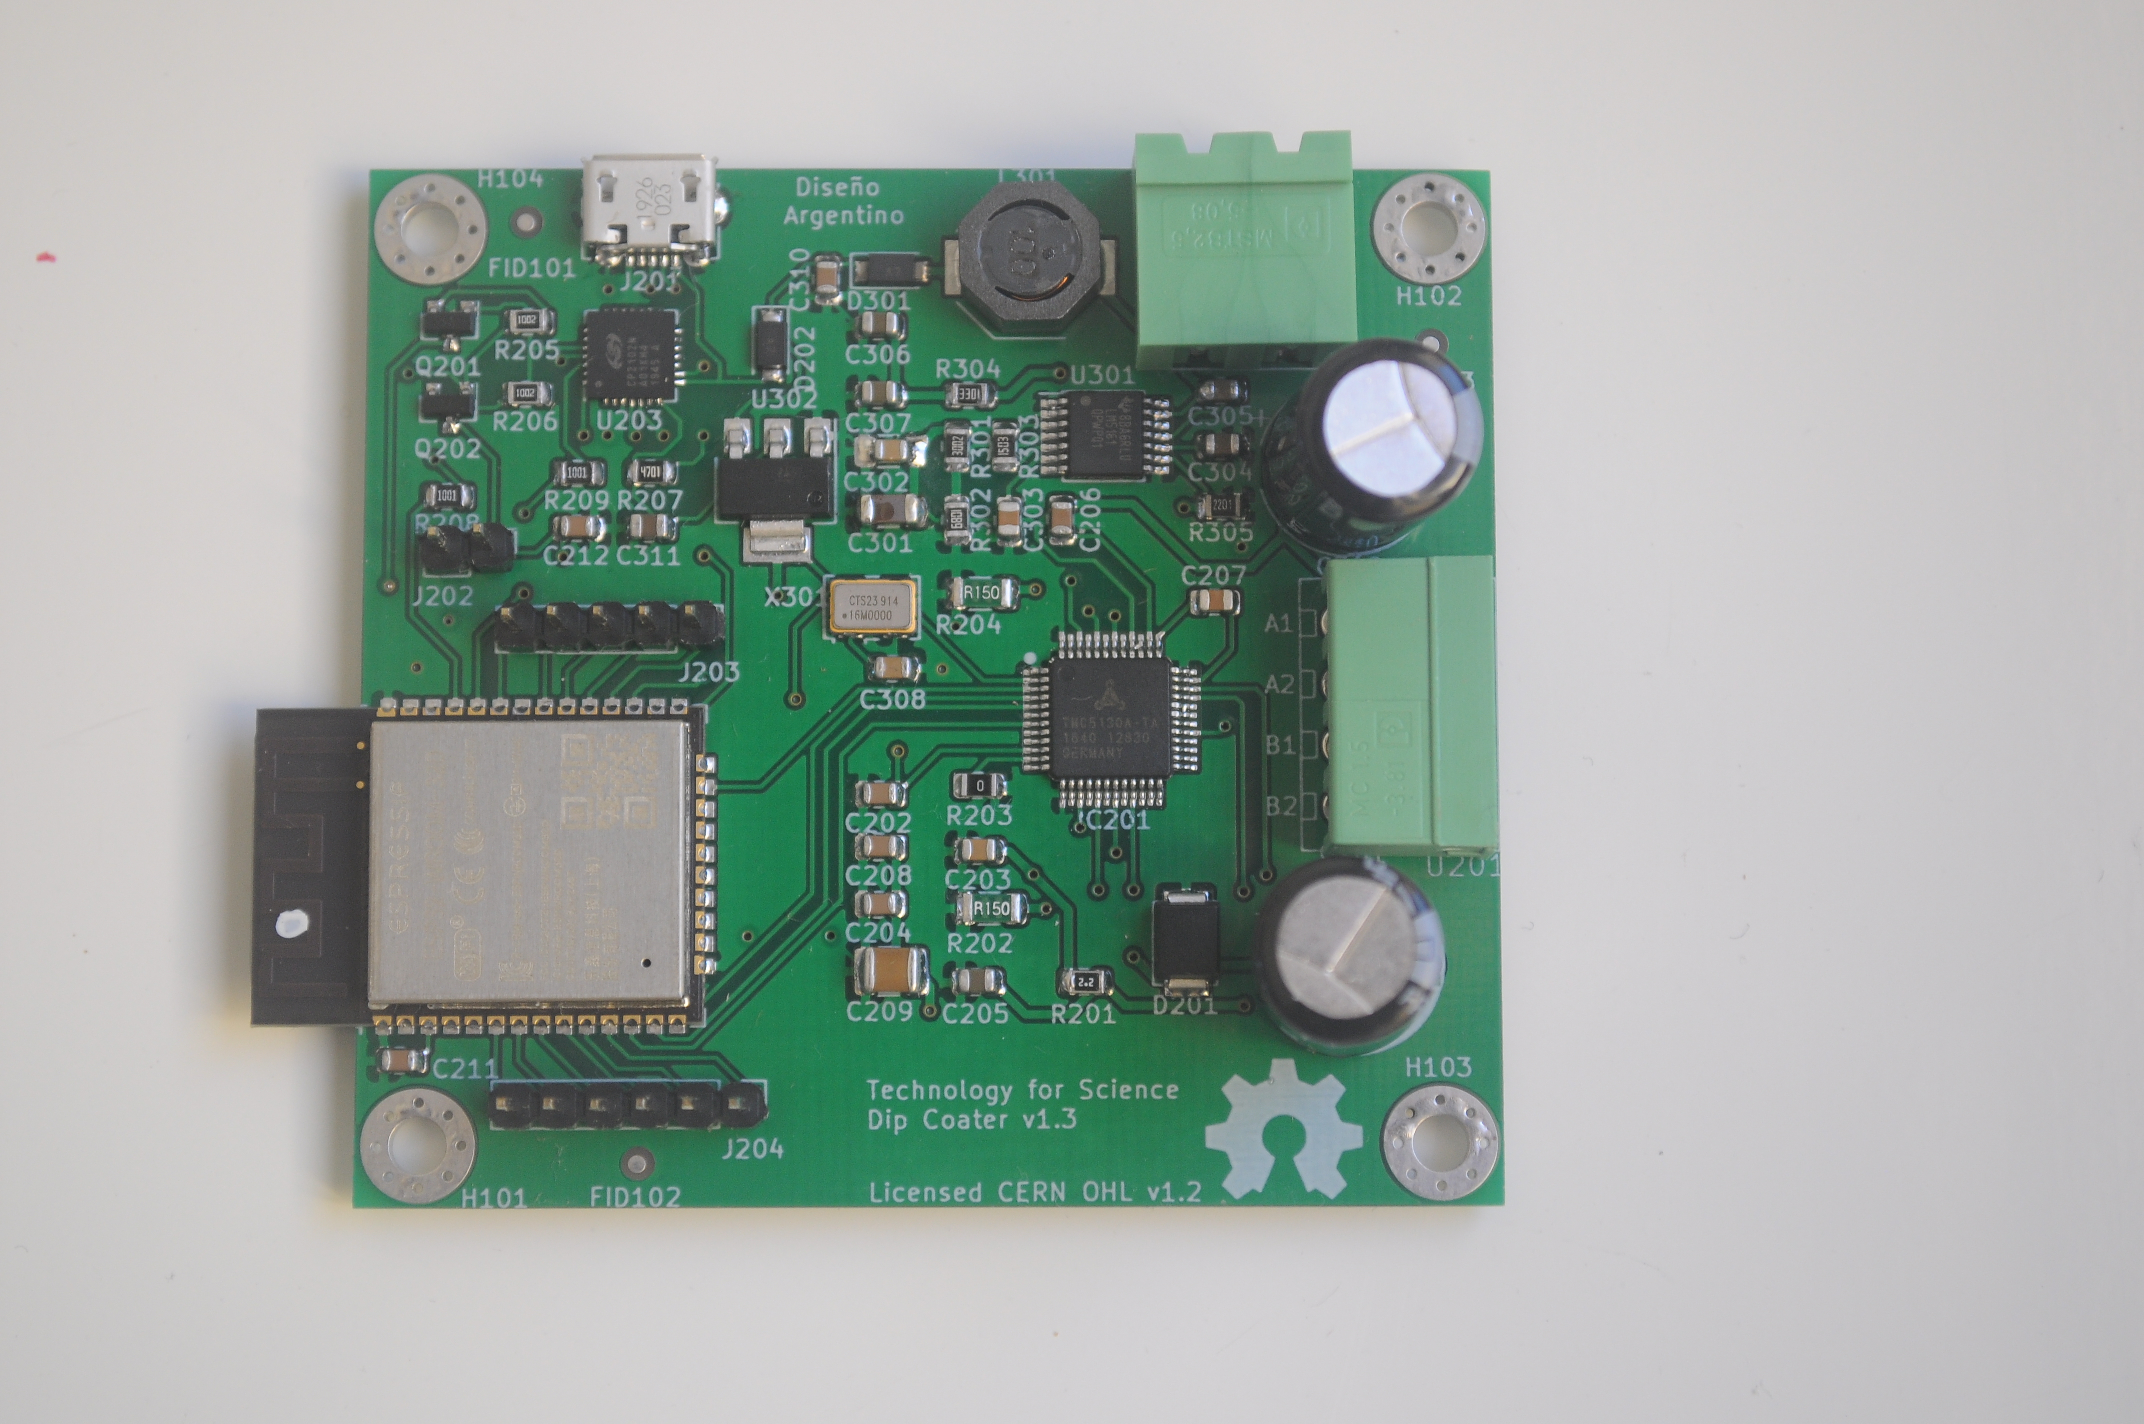
\includegraphics[width=.5\textwidth]{./Figures/dip_real_model.pdf}
	\caption{Placa fabricada MAYER SRL.}
	\label{fig:dip_real_model}
\end{figure}

%----------------------------------------------------------------------------------------
%	SECTION 2
%----------------------------------------------------------------------------------------

\section{Firmware}

\subsection{Capas de abstracción}
\subsection{Framework de trabajo}
\subsection{Módulos principales}



%----------------------------------------------------------------------------------------
%	SECTION 3
%----------------------------------------------------------------------------------------

\section{Estructura mecánica}
\subsection{Fabricación de piezas personalizadas a través de mecanizado CNC}

Como se menciono en la \ref{sec:estructura_mecanica} se utilizó para el software BOBCAD 

\begin{figure}[ht]
	\centering
	\includegraphics[width=.5\textwidth]{./Figures/3d_carro.png}
	\caption{Pieza personalizada para el carro.}
	\label{fig:carro}
\end{figure}

\begin{figure}[ht]
	\centering
	\includegraphics[width=.5\textwidth]{./Figures/3d_estrategia.png}
	\caption{Estrategias de mecanizado en software Bodcad.}
	\label{fig:estrategia}
\end{figure}

\begin{figure}[ht]
	\centering
	\includegraphics[width=.5\textwidth]{./Figures/3d_top.png}
	\caption{Piezas personalizado para sostener estructura superior.}
	\label{fig:estructura_superior}
\end{figure}

\subsection{Modelos 3D y real}

\begin{figure}[ht]
	\centering
	\includegraphics[width=.8\textwidth]{./Figures/3d.jpg}
	\caption{Modelo 3D.}
	\label{fig:mecanica_3d_model}
\end{figure}

\begin{figure}[ht]
	\centering
	\includegraphics[width=.5\textwidth]{./Figures/real.png}
	\caption{Primer prototipo dip coater TECSCI.}
	\label{fig:mecanica_real_model}
\end{figure}
% Chapter Template

\chapter{Ensayos y resultados} % Main chapter title

\label{Chapter4} % Change X to a consecutive number; for referencing this chapter elsewhere, use \ref{ChapterX}

%----------------------------------------------------------------------------------------
%	SECTION 1
%----------------------------------------------------------------------------------------

\section{Pruebas funcionales de hardware y rediseño}
%\label{sec:pruebasHW}

En el presente capítulo se explican los ensayos realizados sobre el prototipo de equipo dip coater, se presentan y analizan los resultados obtenidos y se introducen posibles cambios para próximas versiones.
\subsection{Comunicación con periféricos}

El presente ensayo se realizó para verificar la comunicación entre el microcontrolador ESP32 y el CI TMC5130, como se mencionó en el capítulo \ref{Chapter3} dicha comunicación se establece a través del  protocolo SPI. 

El paquete de datos está definido por un datagrama de 5 bytes, el primer byte define la dirección del registro y los 4 bytes restantes representan el valor. La comunicación con el CI TMC5130  es constante, al encender el equipo se realiza una configuración inicial en donde se escriben todos los registros y luego se realizan operaciones de lectura y escritura para conocer el estado del CI y accionar diferentes tipos de movimientos.

A continuación en la figura \ref{fig:datagrama} se observa la estructura de datos para leer y escribir registros.
\begin{figure}[h]
\centering 
\includegraphics[width=1\textwidth]{./Figures/datagrama.png}
\caption{Datagrama de 40 bits.}
\label{fig:datagrama}
\end{figure}

Las operaciones de lectura y escritura tienen una diferencia, representada por el bit mas significativo de la trama de datos, es decir el bit 39. Cuando la operación es de lectura, y primer byte que representa la dirección del registro no sufre alteración. Cuando la operación es de escritura, hay que establecer en 1 el bit de la posición 39. Por ejemplo si queremos escribir un valor en el registro 0x22, el primer byte del datagrama debería ser 0x22 + 0x80 = 0xA2,  sumar 0x80 representa poner en 1 el primer bit del byte mas significativo del datagrama. 


Para realizar el ensayo se utilizo un analizador lógico USB conectado a la placa electrónica, específicamente sobre los terminales que establecen la comunicación SPI entre el microcontrolador y el CI TMC5130. Se puede observar en la siguiente figur  el banco de pruebas del ensayo.

El procedimiento realizado fue el siguiente:
\begin{enumerate}
\item Conectarse al equipo dip coater con software Putty.
\item Abrir el software del analizador lógico y comenzar registro de datos.
\item Ejecutar comando de lectura del registro 0x2D.
\item Ejecutar comando de escritura del registro 0x2D con valor 100.
\item Ejecutar nuevamente comando de lectura de registro 0x2D y verificar el valor ingresado en el item anterior. 
\end{enumerate}

Se observan a continuación los datagramas capturados en el software del analizador lógico.



Con este ensayo se pudo validar la correcta comunicación entre el microcontrolador y el CI TMC5130 para las operaciones de lectura y escritura de datos.

\section{Pruebas funcionales firmware y rediseño}
\subsection{Tiempo de ejecución de movimientos}

El ensayo se realizó para verificar los parámetros que definen el desplazamiento de la muestra, es decir para verificar que las velocidades y aceleraciones que definen movimientos sean similares a las que surgen del cálculo teórico.

En el capítulo \ref{Chapter3} se detalló la configuración de la rampa de seis puntos que define un movimiento y se mostró la configuración de los parámetros para obtener una rampa de cuatro puntos en donde la etapa de aceleración es igual a la etapa de desaceleración.

Dicha rampa está definida por la siguiente ecuación \ref{eq:movimiento_completo}.

\begin{equation}
	\label{eq:movimiento_completo}
	\vec{x}=\vec{x_o}+\vec{v}(t-t_o)+\frac12 \vec {a} (t-t_o)^2
\end{equation}
%(((2*velocidad)/(aceleración*1000))+(desplazamiento/velocidad))*60*1000  

Por lo tanto, con los valores de aceleración, desaceleración, velocidad y desplazamiento se puede calcular el tiempo teórico necesario para la ejecución de un movimiento.
A continuación en la siguiente tabla \ref{tab:ensayo_comandos} se observan los valores de los parámetros ensayados.

\begin{table}[h]
	\centering
	\caption[Ensayo de tiempo en desplazamientos]{Ensayo de tiempos en desplazamiento}
	\begin{tabular}{c c c }    
		\toprule
		\textbf{Velocidad (mm/min)}     & \textbf{Aceleración-Desaceleración(m/min)} & \textbf{Desplazamiento(mm)} \\
		\midrule
		1  mm/min	 & 	   100-500-1000-2100 m/min2     & 	50 mm 			 	\\		
		10  mm/min   & 	   100-500-1000-2100 m/min2 	& 	50 mm				\\
		100  mm/min  & 	   100-500-1000-2100 m/min2	    & 	50 mm 				\\
		200  mm/min	 & 	   100-500-1000-2100 m/min2	    & 	50 mm 			\\
		500  mm/min	 & 	   100-500-1000-2100 m/min2     & 	50 mm					\\
		800  mm/min	 & 	   100-500-1000-2100 m/min2     & 	50 mm					\\
		\bottomrule
		\hline
	\end{tabular}
	\label{tab:ensayo_comandos}
\end{table}

Para realizar el ensayo se programó una aplicación de prueba que realizaba el siguiente procedimiento:

\begin{enumerate}
\item Configuración de movimiento descendente con valores de velocidad, aceleración y desplazamiento.
\item Ejecución del movimiento y registro del tiempo del sistema.
\item Registro del tiempo del sistema al final del movimiento, cálculo de variación temporal y envío del dato por terminal UART.
\item Configuración y ejecución de movimiento ascendente con sus respectivos registros y envío de dato.
\item Incremento de la tabla hacia nuevos parámetros.
\item Repetición del ciclo.
\item Un ordenador conectado al equipo ejecuta un script de Python que almacena los datos recibidos en un archivo.
\end{enumerate}

En la siguiente figura \ref{fig:tiempo_movimiento_1} se observa en el eje Y el tiempo en ms necesario para ejecutar cada movimiento, los dos puntos cercanos representan el descenso y ascenso con los mismos parámetros de velocidad, aceleración y desplazamiento. El gráfico compara los tiempos teórico respecto a los tiempos registrados. A simple vista no se puede visualizar diferencias significativas entre ambos pares de puntos.

\begin{figure}[h]
\centering 
\includegraphics[width=1.2\textwidth]{./Figures/tiempo_movimiento_1.png}
\caption{Comparación de tiempos teóricos y registrados.}
\label{fig:tiempo_movimiento_1}
\end{figure}

Se presenta a continuación en la figura \ref{fig:error_porcentual_1} un gráfico que representa los errores relativos porcentuales de las mediciones anteriores. Se puede deducir que existe un aumento del error relativo a velocidades altas, con un registro pico  en la velocidad de 800 mm/min. 


\begin{figure}[h]
\centering 
\includegraphics[width=1\textwidth]{./Figures/error.png}
\caption{Error relativo porcentual.}
\label{fig:error_porcentual_1}
\end{figure}
Se concluye con este ensayo que el equipo es muy preciso en la mayor parte del rango para el cual fue diseñado teniendo un error relativo pico de 13\% en las velocidades superiores del rango de funcionamiento.
 
  
\section{Calibración del equipo}
\label{sec:calibración}
\subsection{Desplazamiento lineal y micro pasos}

Este ensayo se realizó para definir y ajustar la constante de desplazamiento que relaciona los micros pasos realizados por el motor con la distancia de desplazamiento del carro. La misma es una constante que está definida por las dimensiones del tornillo, es decir el paso del mismo,  sobre el cual de desplaza el carro.

Para realizar las mediciones se utilizó un comparador digital de la marca Asimeto\citep{web_asimeto} el cual puede observarse en la figura \ref{fig:micrometro}, el mismo tiene una resolución de 0.0001 mm y permite desplazamientos de 0 a 50 mm.


\begin{figure}[h]
\centering 
\includegraphics[width=0.3\textwidth]{./Figures/micrometro.png}
\caption{Comparador digital Asimeto.}
\label{fig:micrometro}
\end{figure}

El ensayo consistió en medir seis desplazamientos sucesivos de 1 mm sobre el carro de manera descendente y luego de manera ascendente. Este ensayo es importante porque permite corregir la unidad de conversión de micro pasos a milímetros que utiliza el CI TMC5130 para realizar todos los movimientos. 
En la subsección \ref{subsec:calibracion} se mencionó la macro \textit{MACHINE STEPS PER MILLIMETER} definida en el archivo hardware.h que surgió de este ensayo. 

En la figura \ref{fig:desplazamiento_lineal} se observa el banco de medición donde se visualiza el comparador Asimeto apoyado sobre una base metálica independiente con la punta del mismo en contacto directo con el carro de desplazamiento.

\begin{figure}[h]
\centering 
\includegraphics[width=0.5\textwidth]{./Figures/desplazamiento_lineal.png}
\caption{Ensayo de desplazamiento lineal.}
\label{fig:desplazamiento_lineal}
\end{figure}


Para iniciar el ensayo se presiona el botón \textit{origin} del comparador para poner en cero la medida, la sensibilidad del mismo es tan grande que es difícil lograr 0,000 mm debido a la acción misma  de apretar el botón. Luego se realizan movimientos descendentes de 1 mm y se registran los datos.
En la siguiente tabla \ref{tab:ensayo_desplazamiento_des} se muestran los resultados obtenidos.

\begin{table}[h]
	\centering
	\caption[Ensayo de desplazamiento]{Ensayo de desplazamiento lineal descendentes}
	\begin{tabular}{l c c }    
		\toprule
		\textbf{Posición absoluta}     & \textbf{Desplazamiento relativo} & \textbf{Error Relativo} \\
		\midrule
		0,058 mm	& 	        	& 	 			 	\\		
		1,051 mm    & 	0,993 mm    	& 	0,007				\\
		2,035 mm 	& 	0,984 mm	    & 	0,016 				\\
		3,034 mm	& 	0,999 mm	    & 	0,001 			\\
		4,054 mm 	& 	1,02 mm         & 	-0,020					\\
		5,039 mm 	& 	0,985 mm	    & 	0,015					\\
		5,998 mm 	& 	0,959 mm        & 	0,041 			\\
		\bottomrule
		\hline
	\end{tabular}
	\label{tab:ensayo_desplazamiento_des}
\end{table}

De igual manera se confecciona la siguiente tabla \ref{tab:ensayo_desplazamiento_asc} para los movimientos ascendentes.
 
\begin{table}[h]
	\centering
	\caption[Ensayo de desplazamiento]{Ensayo de desplazamiento lineal ascendentes}
	\begin{tabular}{l c c }    
		\toprule
		\textbf{Posición absoluta}     & \textbf{Desplazamiento relativo} & \textbf{Error Relativo} \\
		\midrule
		0,02 mm	& 	        	& 	 			 	\\		
		0,939 mm    & 	0,019 mm    	& 	0,081	\\
		1,931 mm 	& 	0,992 mm	    & 	0,008 	\\
		2,929 mm	& 	0,998 mm	    & 	0,002 	\\
		3,923 mm 	& 	0.994 mm        & 	0,006	\\
		4,923 mm 	& 	1 mm	    	& 	0		\\
		5,911 mm 	& 	0,988 mm        & 	0,012 	\\
		\bottomrule
		\hline
	\end{tabular}
	\label{tab:ensayo_desplazamiento_asc}
\end{table}


Para corregir el valor de micro pasos por milímetros de desplazamiento se utilizo el siguiente procedimiento.
\begin{enumerate}
\item Realizar un promedio de los 6 errores relativos ascendentes y descendentes.
\item Ajustar el valor inicial de micro pasos con los respectivos errores. 
\item Realizar un promedio entre el valor corregido ascendente y el valor corregido descendente.
\end{enumerate}


Inicialmente al comenzar el ensayo la macro \textit{MACHINE STEPS PER MILLIMETER}  estaba definida con un valor de 12737 micro pasos por milímetros, luego de sucesivas correcciones la macro quedo definida en 12932 micro pasos por milímetros.
Este ensayo se repitió cinco veces hasta llegar a los valores presentados en las tablas anteriores, en donde se observó que el porcentaje promedio de los errores relativos no afectaba en las décimas de milímetros.

\section{Caso de prueba}
\section{Prueba de campo con personal capacitado}

El siguiente ensayo consistió en una prueba completa del equipo dip coater con personal capacitado del Instituto de Nanosistemas.
La prueba que se llevo a cabo consistió en realizar el primer \textit{thin films} del equipo, se utilizó un wafer de silicio como sustrato y una solución de dioxido de titanio disuelto en etanol para formar un film de nanoparticulas de titanio.

\begin{figure}[h]
\centering 
\includegraphics[width=0.5\textwidth]{./Figures/prueba_b.jpg}
\caption{Ensayo completo en laboratorio.}
\label{fig:desplazamiento_lineal}
\end{figure}


\begin{figure}[h]
\centering 
\includegraphics[width=0.5\textwidth]{./Figures/prueba_a.jpg}
\caption{Ensayo con wafer de silicio.}
\label{fig:desplazamiento_lineal}
\end{figure}


 
% Chapter Template

\chapter{Conclusiones} % Main chapter title

\label{Chapter5} % Change X to a consecutive number; for referencing this chapter elsewhere, use \ref{ChapterX}


%----------------------------------------------------------------------------------------

%----------------------------------------------------------------------------------------
%	SECTION 1
%----------------------------------------------------------------------------------------
En esté capítulo se presentan las conclusiones principales sobre la fabricación de un equipo dip coater, se detallan los logros mas importantes del trabajo y se mencionan algunos puntos para mejorar en futuros trabajos, por último se plantean las planes inmediatos de desarrollo, fabricación y comercialización del equipo.

\section{Resultados obtenidos }


El principal hito del trabajo fue fabricar un MVP (producto mínimo viable) de equipo dip coater que cuente con las características suficientes para satisfacer las demandas de primeros usuarios. Podemos entonces señalar los siguientes logros en el desarrollo del presente trabajo: 
\begin{itemize}
\item Se logró diseñar y fabricar un lote de cinco unidades con la primer versión de placa electrónica.
\item Se desarrolló un firmware modular que cumple todos los requerimientos y permite incorporar nuevas funcionalidades sin cambios importantes en la estructura.
\item Se logró generar la capacidad técnica suficiente para fabricar las piezas mecanizadas del primer equipo.  
\end{itemize} 
 


Lamentablemente la planificación original no pudo ser sostenida, abarcar íntegramente la fabricación de un MVP fue demasiado trabajo para los tiempos y recursos establecidos. Existieron retrasos en tareas en las cuales el autor no contaba con los conocimientos necesarios para su correcta definición, principalmente en todo el diseño y fabricación mecánica. Sin embargo, surge de este trabajo una base de conocimiento importante que permite comenzar con el desarrollo y la fabricación de otro MVP en tiempos mas acotados y con una planificación mas certera. 


%----------------------------------------------------------------------------------------
%	SECTION 2
%----------------------------------------------------------------------------------------
\section{Próximos pasos}

Se plantean los siguientes puntos fundamentales para el futuro inmediato del equipo:  

\begin{itemize}

\item Se fabricará un lote nuevo de diez placas. 

\item En lo inmediato se incorporará un módulo de software para el registro de parámetros de humedad y temperatura , que será integrado con el desarrollo futuro de una cámara de humedad compatible con este equipo.

\item Durante el mes de junio del presente año investigadores del INS (Instituto de Nanositemas) llevarán a cabo ensayos para caracterizar el equipo. El ensayo contemplará la generación de cincuenta \textit{films} sobre soluciones químicas de \ce{TiO2} y \ce{SiO2} caracterizadas a través del método XRR (reflectometría de rayos-X). Surgirá de este ensayo un documento técnico con los resultados obtenidos.  
 
\item A través de un arreglo de cooperación se entregarán dos equipos a usuarios calificados para realizar pruebas funcionales y evaluar su satisfacción. Se realizarán cambios de ser necesario.


\item Se trabajará en conjunto con un diseñador industrial para convertir este MVP en un producto comercial de la empresa TECSCI.

\end{itemize}


 

%----------------------------------------------------------------------------------------
%	CONTENIDO DE LA MEMORIA  - APÉNDICES
%----------------------------------------------------------------------------------------

\appendix % indicativo para indicarle a LaTeX los siguientes "capítulos" son apéndices

% Incluir los apéndices de la memoria como archivos separadas desde la carpeta Appendices
% Descomentar las líneas a medida que se escriben los apéndices

%\include{Appendices/AppendixA}
%\include{Appendices/AppendixB}
%\include{Appendices/AppendixC}

%----------------------------------------------------------------------------------------
%	BIBLIOGRAPHY
%----------------------------------------------------------------------------------------

\Urlmuskip=0mu plus 1mu\relax
\raggedright
\printbibliography[heading=bibintoc]

%----------------------------------------------------------------------------------------

\end{document}  
